\documentclass{tufte-book}
\hypersetup{colorlinks}

\usepackage{amsmath}

% Set up the images/graphics package
\usepackage{graphicx}
\setkeys{Gin}{width=\linewidth,totalheight=\textheight,keepaspectratio}
\graphicspath{{graphics/}}

\title{Setting the Stage for Interaction}
\author[Drew Harry]{Drew Harry}
% \publisher{}

%\date{24 January 2009}  % if the \date{} command is left out, the current date will be used

% The following package makes prettier tables.  We're all about the bling!
\usepackage{booktabs}

% The units package provides nice, non-stacked fractions and better spacing
% for units.
\usepackage{units}

% The fancyvrb package lets us customize the formatting of verbatim
% environments.  We use a slightly smaller font.
\usepackage{fancyvrb}
\fvset{fontsize=\normalsize}

% Small sections of multiple columns
\usepackage{multicol}

% Provides paragraphs of dummy text
\usepackage{lipsum}

% Provides rotated tables + table labels, which I might use.
\usepackage{rotating}

% some circles I need
\usepackage{wasysym}

\usepackage{multirow}

%%
% Prints argument within hanging parentheses (i.e., parentheses that take
% up no horizontal space).  Useful in tabular environments.
\newcommand{\hangp}[1]{\makebox[0pt][r]{(}#1\makebox[0pt][l]{)}}

%%
% Prints an asterisk that takes up no horizontal space.
% Useful in tabular environments.
\newcommand{\hangstar}{\makebox[0pt][l]{*}}

%%
% Prints a trailing space in a smart way.
\usepackage{xspace}

% Inserts a blank page
\newcommand{\blankpage}{\newpage\hbox{}\thispagestyle{empty}\newpage}

% Generates the index
\usepackage{makeidx}
\makeindex


\begin{document}
	
\frontmatter

\maketitle

\tableofcontents
\listoffigures
\listoftables

\mainmatter

\chapter{Introduction}
\label{ch:intro}
% need to open with a 


As researchers first started to build technology to help us communicate with other people at a distance, a consensus on what our systems should aspire to do quickly arose: computer mediated communication systems should focus on recreating the experience of being face-to-face with another person. The best system, in this model, is one that seems to disappear in the same way that the best window makes us feel like there is nothing between us and what is on the other side of the glass. Since the early 1970s, it has seemed like we have always been on the verge of a utopian environment where distance disappears and we interact as richly with friends, family, and colleagues around the world as we do with someone sitting in the same room. \citep{Egido:1988vq} And yet, like the paperless office \citep{Sellen:2001uk}, this future has failed to materialize. We can interpret this in two ways: either our tools have failed to deliver on the promise of a ``being there'' level experience or our persistent selection of non-``being there'' experiences reveals a broad desire for a different vision of computer mediated communication. As with \citet{Hollan:1992tz}, I will argue the latter case. In particular, I will focus on how  computer-mediated-communication tools can complement existing interaction contexts. I will show through a series of design projects and studies where we might find ways to create experiences that meet the challenge of being ``beyond being there''; experiences that are compelling precisely because they are trying to be something other than just a face-to-face presence with others.

To introduce this design space, I describe the broader context of computer-mediated-communication systems and why work has long focused on the ``being there'' approach to design. I will discuss approaches described in the literature for thinking about the different design strategies one might employ when trying to build new systems with a ``beyond being there'' approach in mind.

% My research has focused on designing, building, deploying, and observing the use of computer mediated communication systems that complement existing communication technologies and face-to-face interaction. In this dissertation, I will introduce a new theoretical framework for thinking about this category of design and trace that theoretical perspective through a series of design projects in different problem domains. 

% might also be able to deploy a ref to Nilles, J., 1988. Traffic reduction by telecommuting: A status review and selected bibliography. Transportation Research Part A: General. Available at: http://linkinghub.elsevier.com/retrieve/pii/0191260788900088.

\section{Being There}
Core to the argument that computer-mediated-communication should simply recreate face-to-face interactions as transparently as possible is the notion that face-to-face interaction is the best we can hope for. Depending on your perspective, it may seem either heretical or obvious to claim that that we might prefer non-face-to-face interaction in certain situations. We can look to research on media selection preferences to consider the evidence.

Since computer-mediated-communication became technically viable, there has been broad interest in understanding the relative properties of speech, video, and text, as well more esoteric (and largely ignored) modalities like real-time handwriting transmission. \citep{Williams:1977p682} This stream of work can be traced back to \citet{Ochsman:1974vu}, who studied pairs of students coordinating on concrete tasks like scheduling, way-finding, and physical part identification using different sorts of communication tools. This early work focused on measuring which channels were most effective for tasks, and primarily recommended that adding voice provided the biggest improvement in performance. This type of work has continued, with researchers expanding their view beyond task performance to trust formation \citep{Bos:2002p256}\citep{Toma:2010p347} and deception \citep{Hancock:2004p314}.

% also cite the chapanis sci amer article? it's better and a little more broad

Much of this work takes place in an experimental psychological tradition, which focuses on controlled lab contexts for studying communication behaviors. As a research context, this leaves much to be desired in studying the complex \emph{in situ} decisions that people make about communication. Outside of lab contexts, we are not assigned a specific tool for a specific task. Instead, we make nuanced and highly contextual choices about what sorts of tools to use in different communication situations. If we accepted the idea that ``being there'' was a primary motivation, we would expect to see people prioritizing tools that were the most like ``being there'' among the available options. This spectrum is also sometimes characterized as ``media richness'' per \citet{Daft:1986p1548}, in which the most rich media are those that are most like being face-to-face and that people will prefer richer tools over less rich tools. Instead, researchers have found repeatedly that in non-lab situations, people frequently choose less rich media over more rich options. \citep{Scholl:2006p210} If richness alone does not predict people's real-life communication media selection decisions, it suggests that other features of a communication situation might also be relevant and that there exist other priorities than just a desire for ``being there''.

% there are many other takedowns of media richness theory. Could expand those here.
% try to find some more people who find what scholl finds. I know there's lots but I don't have a handy list right now. 

Communication situations are defined by the complex interplay of the features of the communication tools in use and the setting, people involved, purpose, and norms. The non-technical components of the setting will be discussed in more detail in Chapter \ref{ch:background}, but our discussion here will focus on the nature of the medium itself. We can turn to \citet{Brennan:1991wk} as a starting point for other ways we might organize and understand the properties of different sorts of communication media. These aspects of a medium play a large part in how it's used, and help explain the sorts of results seen in studies like \citet{Scholl:2006p210}.

\begin{description}
\item [Reviewability]{Are records of past interactions easily accessible? Who has access to them?}
\item [Revisability]{How are messages constructed? Do you have time to revise a message before it is sent? Can messages be edited or retracted?}
\item [Synchronicity]{Are messages responded to rapidly, or are there longer gaps between messages?}
\item [Sequentiality]{Does the system support multiple simultaneous conversations, or must all contributions fit into a single shared stream?}
\item [Identity]{How are people represented, and what information is made available about each person?}
\item [Mobility]{In what sorts of spaces can this medium be used? What do we expect about the contexts of other people using the system?}
\end{description}


We can evaluate both mediated and non-mediated experiences on each of these axes. Face to face communication, for example, has no reviewability or revisability with high synchronicity, high sequentiality, and high levels of identity disclosure. In the spirit of acting in a complementary way, most of the work described in this thesis attempts to occupy different points in this design space to best complement face to face experiences and those mediated experiences that attempt to mimic face to face interaction. Furthermore, I will argue that different experiences can effectively co-exist, each complementing the strengths and weaknesses of other mediated and non-mediated channels.

% also link to facetime?
The continued focus on ``being there'' designs by much of the communication industry, Cisco's Telepresence systems (see figure \ref{fig:cisco-telepresence}) and Apple's Facetime (see figure \ref{fig:facetime}), and Google Hangouts being major examples, has blinded us to the potential of other approaches. They reinforce the framing of mediated communication as something less rich and less effective than face to face. Part of this is about scale; one on one or small group interactions are hard to improve. But a closer inspection of face-to-face interaction among groups of more than five people reveals a number of potential challenges:


\begin{itemize}
\item Not all people are equally capable of convincing performances in face-to-face interaction. This can be the result of a variety of factors, including (but not limited to) a lack of confidence in contributing in a specific context, a lack of skill with language, or the impact of a power imbalance in the situation. Many of these can be mitigated in mediated contexts\citep{Siegel:1986ve}, although mediated contexts have their own distinct performance challenges.
\item Simultaneous contribution in face-to-face situations are often viewed as impolite and are generally normatively discouraged. Particularly in large groups, this represents a pressure against contribution and requires a certain amount of overhead to negotiate turn-taking gracefully.
\item Participation in face-to-face contexts usually discloses significant information about someone's identity, while in mediated contexts there are a variety of approaches to limiting disclosure of identity information while still being an active participant.
\item Face-to-face interactions are traditionally ephemeral and difficult to record; mediated interactions are usually quite easy to record, even those that mimic face-to-face interaction. 
\end{itemize}


% I want to be able to cite the commercials, but it's a nightmare finding any information about them that might make them citable like where they appeared, when they appeared, who directed them, etc.


\begin{marginfigure}
	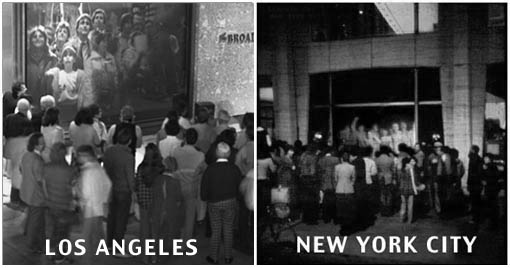
\includegraphics{figures/hole_in_space.jpg}
	\caption{Photos of the Hole in Space exhibit sites in Los Angeles and New York City.}
	\label{fig:hole-in-space}
\end{marginfigure}

\begin{marginfigure}
	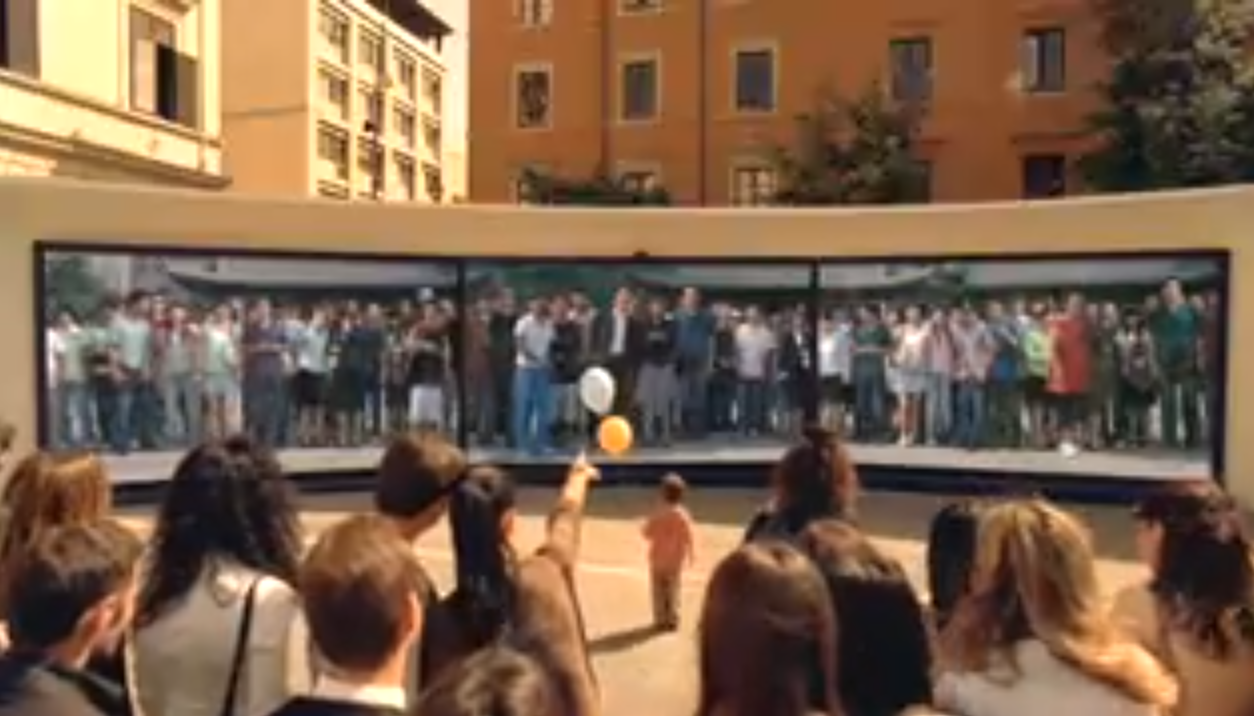
\includegraphics{figures/cisco-telepresence.png}
	\caption{Still from a Cisco Telepresence advertisement, centered on connecting an Italian piazza with a Chinese square with a seamless window.}
	\label{fig:cisco-telepresence}
\end{marginfigure}

% Despite these challenges, there's still an undeniable magic to the pursuit of recreating face-to-face communication at a distance. This magic is most poetically captured in the famous ``Hole in Space'' \citep{HoleinSpace:1980vn} piece, visually and audibly connecting a storefront in Los Angeles and New York in a way that seemed to make distance disappear. This vision is not simply aspirational, either. Tools to communicate with physically distant people either with audio alone or with an added video connection play a role in the daily lives of millions of people. This desire to experience ``being there'' with someone else is powerful and compelling.


\begin{marginfigure}
	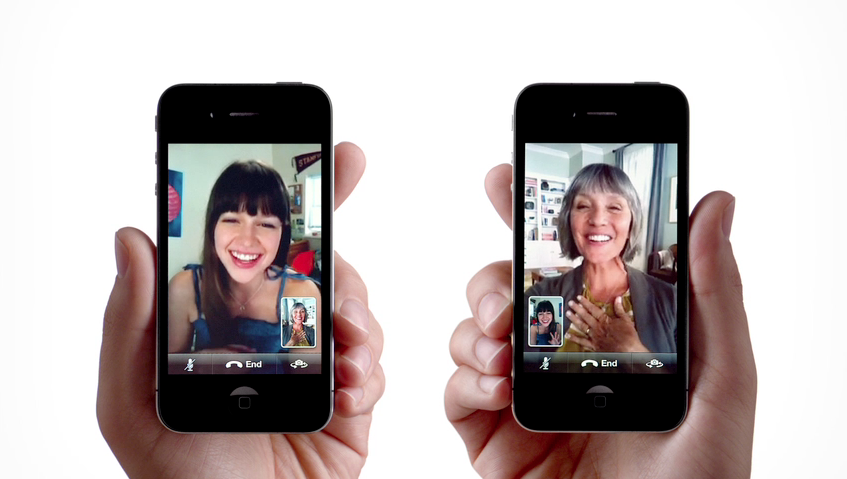
\includegraphics{figures/iphone-face-to-face.png}
	\caption{Still from an Apple advertisement demonstrating the Facetime feature to enable mobile video conferencing.}
	\label{fig:facetime}
\end{marginfigure}




\section{Complementary Communication}
This thesis addresses the design space of complementary communication systems. By this, I mean systems that aim to create a communication context shared by a group of people who are sharing some kind of experience like a presentation, performance, or discussion. Viewed this way, complementary communication systems are as old as whispering to someone sitting next to you or passing notes to a classmate. The addition of powerful personal communication technology to our everyday interactions have increased the opportunities we have to create complementary communication contexts as well as radically increased the reach a complementary communication system might have. In this context, how should we think about these sorts of systems? What goals should we have for them? In what contexts do they make sense? In particular, how should we think about the relationship between a complementary communication system in a face to face context? Is complementing a face to face interaction the same as complementing a mediated interaction?


In their famous paper, \citet{Hollan:1992tz} introduce the ``beyond being there'' approach. They argue that seeking to recreate the experience of ``being there'' was in a way an abdication of our responsibility as designers that left an important design space un-explored. In particular, they urge us to think less about ways to minimize the experience of mediation in communication, but to look instead for ways that mediation can add value to interactions. To take this perspective seriously, we need to shift away from a view of face-to-face interaction as being always better than interactions mediated by technology and instead think critically about potential limitations and challenges with face-to-face interaction and potential benefits that mediation can offer. 

\begin{marginfigure}
	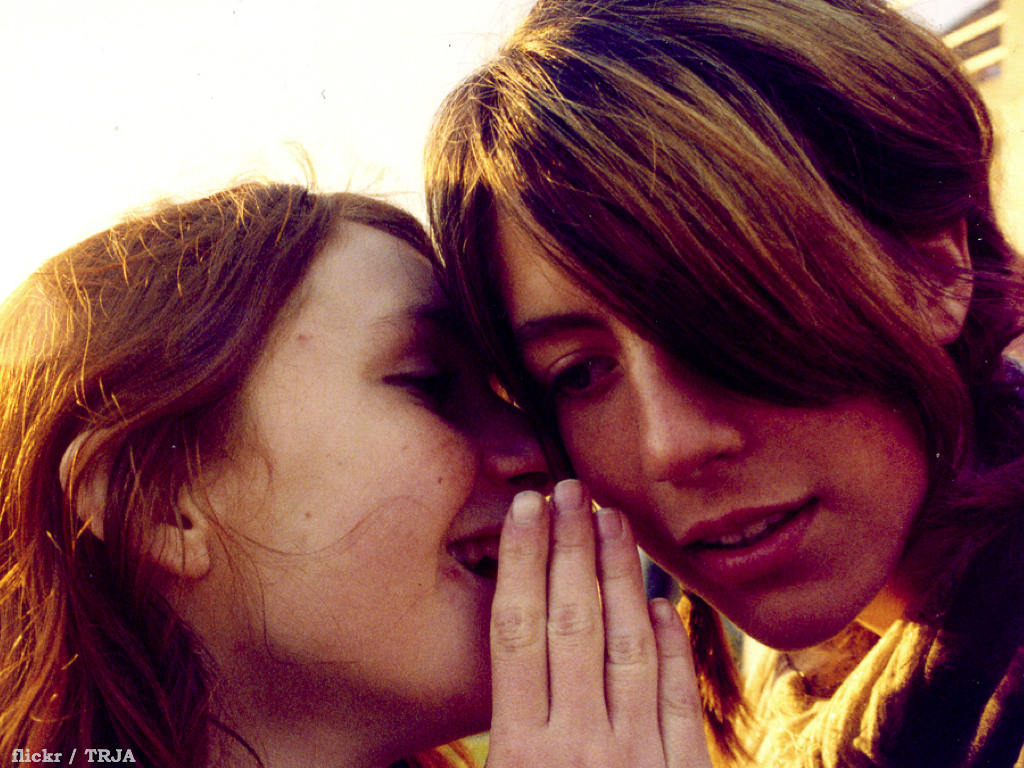
\includegraphics{figures/whisper.png}
	\caption{The original complementary communication experience.}
	\label{fig:whisper}
\end{marginfigure}


Although Hollan and Stornetta focus on creating mediated experiences that rival or surpass face-to-face experiences, in my work I show that we don't have to choose one approach or the other. If we accept the argument that being face to face is not \emph{a priori} the best experience, the strategy I employ is to add complementary communication platforms that can be used simultaneously with face-to-face communication or mediated platforms that mimic face to face interaction.


\begin{marginfigure}
	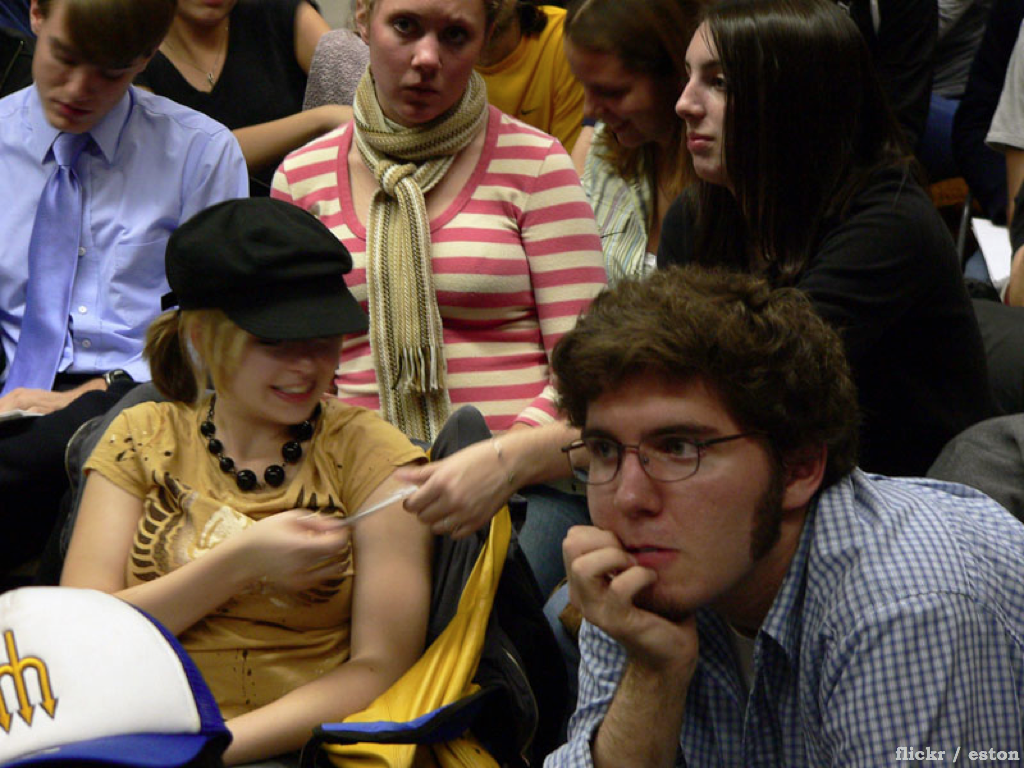
\includegraphics{figures/note-passing.png}
	\caption{The first complementary communication technology.}
	\label{fig:notes}
\end{marginfigure}


This easy equivalence between face-to-face communication and mediated imitations may seem unlikely; why should we accept that systems used in coordination with audio or video conferencing would be similar to those used to coordinate face-to-face? I will argue that a system that can effectively complement face-to-face interaction when its users could simply set it aside and rely on the (presumed superior) affordances of unfettered verbal communication likely has something to tell us about both design and face-to-face interaction more generally. If these systems can provide value in face-to-face contexts, I will show that they also provide value (perhaps even more value) when used to complement systems that seek to create experiences \emph{like} being face-to-face. Furthermore, true ``distributed'' situations are becoming less common. Heterogenous configurations where some people are co-located and others are remote and possibly alone are becoming more common. In these contexts, a system that doesn't operate effectively between co-located users is unlikely to be broadly useful, and would suffer from the disenfranchising effects we see for people who ``dial in'' to a local meeting. Thinking broadly about systems that complement both face-to-face and audio/video sharing will more efficiently lead us to systems effective in both contexts than treating them as separate cases.

\begin{marginfigure}
	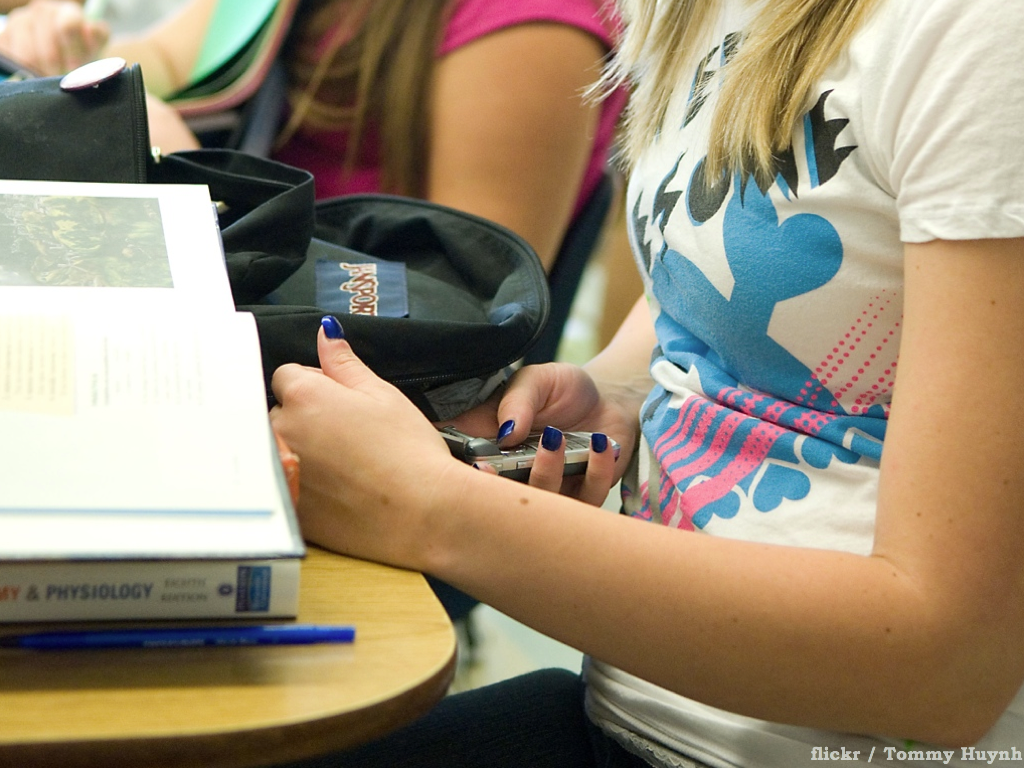
\includegraphics{figures/texting.png}
	\caption{Person to person text messaging extends the reach of something like note passing to include anyone with a phone. Phones also support multi-party conversations, increasing the size of the audience for complementary communication systems.}
	\label{fig:texting}
\end{marginfigure}




% think about listifying this section

% Many of these challenges are common sense, even if they are frequently forgotten when people argue for recreating face-to-face experiences. Face-to-face communication requires relatively explicit turn-taking; multiple speakers in a group make them all largely unintelligible. In mediated environments like chat, simultaneous conversation threads can easily co-exist for long periods of time. There are major identity implications to face-to-face communication. It is difficult to conduct any face-to-face communication without revealing significant information about your identity. In mediated contexts, there are techniques ranging from anonymity to pseudonymity to limit identity disclosing information. Participation in non-mediated interactions is ephemeral, while mediated interaction can easily be archived and represented either in context or after the fact. Participation in face-to-face situations can be limited by confidence, but mediated participation tends to be more disinhibited. \citep{Siegel:1986ve}

% is this a second order effect?
% For a variety of reasons, the power dynamics in social situations are more easily subverted in mediated environments. 

This dissertation is organized around a series of ``primary'' contexts for which I design a particular complementary communication system that enhances the overall experience. Metrics and evaluation strategies vary for each of these pieces, but each project shares a deep interest in trying to fill in the gaps of the ``primary'' interaction space by using the particular strengths of some additional mediated communication system. The goal of these interventions is to create environments where people have ways to express themselves non-verbally in addition to whatever existing communication channels exist, often audio, sometimes visual. By adding mediated communication channels to other existing channels, we can focus each channel on its primary affordances and let it do what it does best while letting the complementary communication channels fill in the gaps.


\section{From Channel To Stage}

Platforms for discussion and commenting that are outside official discourse channels have widely been referred to as ``backchannels.''  Backchannels, traditionally defined, create a space where audience members to some ``front channel'' can share information with each other, typically about the content of the front channel. \sidenote{This is in contrast with the traditional technical use of ``backchannel'', which refers to the verbal and non-verbal cues that non-speaker give a speaker during a conversation. In this usage, backchannel was a type of communication, not an actual dedicated distinct channel the way it is in this context.} This metaphor is an apt description of much of the prior work in this space, like \citep{Cogdill:2001fp,Yardi:2006uk,mccarthy_digital_2004,Rekimoto:1998jy}. I have found, however, that it is not as useful for understanding the systems I will present in this thesis. Instead of using channels, I will argue for ``stages,'' and instead of a front/back separation, I will shift to a main/side distinction. \sidenote{Parts of the section to follow are adapted from \citep{Harry:2012df}.}


In a traditional backchannel configuration, audience members can view the front channel and have a variety of backchannels available to them, each with different sized audiences and affordances. This is represented in Figure \ref{fig:front-back-channel}. Presenters, on the other hand, often have a very hard time staying aware of backchannel content if they are aware of it at all. This asymmetry gives the backchannel its outsider flavor and can lead to disrespectful and unproductive content \citep{boyd:Yo36SNyj}. This is widely recognized as a major problem with backchannels. In this way, the front/back distinction is an accurate description of existing systems, but not a situation I seek to recreate. \sidenote{Of course, there may be contexts where the front/back distinction is valuable. But since that is the predominant structure for existing tools, there are many more options for supporting that approach so I don't give it much attention in this thesis.} Mitigating this sense of separation is a major design goal in my work.





% In this configuration, the front/back channel distinction is a useful one because in a very practical sense the backchannel is usually somewhat covert or hidden and participants in the backchannel rarely have the ability or opportunity to communicate on the front channel. \sidenote{This paragraph and the rest of this section are largely from \citep{Harry:2012df}.} 

% I wonder if it's worth putting some examples here? I thiiink we can get away without, but might help ground people's thinking.

% Although this front/back channel metaphor works in situations where audience members have no access to the front channel, it is less effective in situations where the backchannel is intended to influence the front channel. 

% As will be discussed in the related work, much recent work is focused on bridging these front and back spaces and I argue through the work presented in this thesis that a new metaphor is useful for understanding how these parallel communication spaces can be configured.

To enable this shift, we need to re-imagine the nature of social interaction in these sorts of spaces. A channel metaphor implies a clear split between those empowered to broadcast, and an audience who receives that broadcast. It also has implications for how attention is managed; channels imply a model of binary attention. To find an alternative, I turn to \citet{goffman_presentation_1959} for his description of \emph{stages} to illuminate this new sort of situation. He uses the example of a waiter behaving politely with a problematic customer and then walking into the kitchen and complaining to the cook about the customer's difficult behavior. Each interaction is performative and represents the waiters' competence at performing his role appropriately for different audiences in a different setting. In the waiter example, these audiences are disjointed, and the door into the kitchen represents a gateway between the ``front'' performance space with customers and the ``back'' performance space among restaurant staff. The notion of stages shifts our attention from spaces where a small number of people can broadcast information to many recipients (like a lecture hall or conference) and instead focuses on negotiated sites of performance like the restaurant dining room and kitchen, where people can perform different aspects of their identity for different audiences. This intermediate state is shown in Figure \ref{fig:front-back-stage}. In this model, the back stage still lacks accessibility for much of the audience, and is not easily perceived by performers on the front stage.

\begin{marginfigure}
	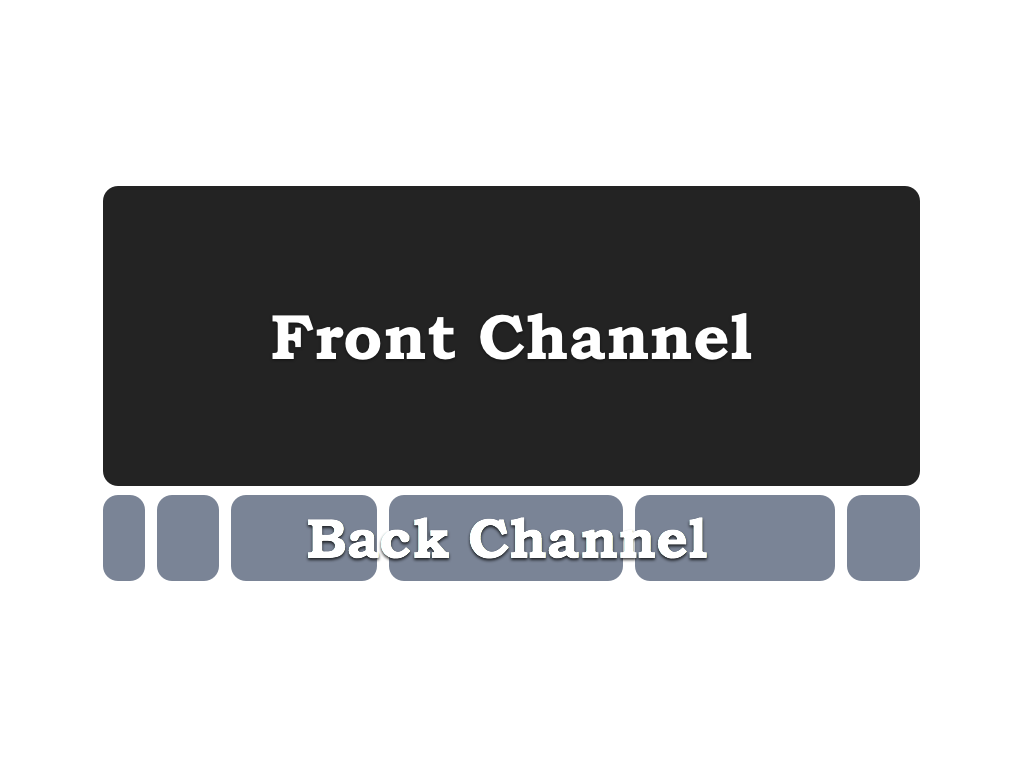
\includegraphics{figures/front-back-channel.png}
	\caption{The conceptual model inherent in a front/back channel configuration.}
	\label{fig:front-back-channel}
\end{marginfigure}

\begin{marginfigure}
	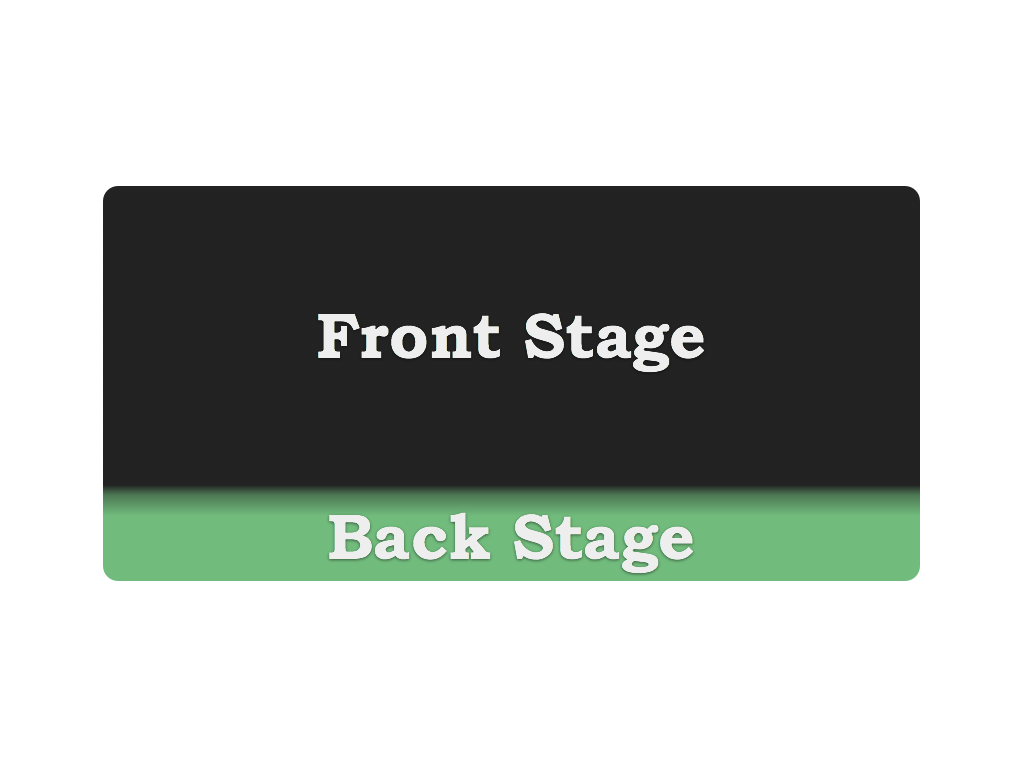
\includegraphics{figures/front-stage-back-stage.png}
	\caption{The transition from channels to stages; brings the audience closer to the performer and increases the visibility of the back stage.}
	\label{fig:front-back-stage}
\end{marginfigure}

This notion of stages is a useful metaphor to replace channels. Unlike channels, where audiences are basically invisible to the performer, stages bring the audience and performer together and create a context in which they are mutually aware of each other. Stages also shift from the notion of a small group of broadcasters and a large group of receivers, to a context where there is the potential for different performers at different moments. The notion of stages also more actively recognizes the way that audiences to a performance are themselves constantly performing in small ways, while a channel metaphor limits the audience to simply receiving a broadcast. This comprises both small performances and the potential for substantial performances. In a large lecture hall, the nature of the individual performance is not that precise. If there is an open laptop policy, audience members might be checking their email or engaging in an official backchannel.  They are able to, as Goffman says, ``get away with going away," because the act of \emph{going away} is an expected part of the front stage performance. But a shift from channels to stages is important in recognizing that even as audience members, looking at a laptop screen instead of the teacher is a sort of small performance. Furthermore, a student may raise their hand and ask a question of the teacher, thus assuming a larger role in the main stage. 

\begin{marginfigure}
	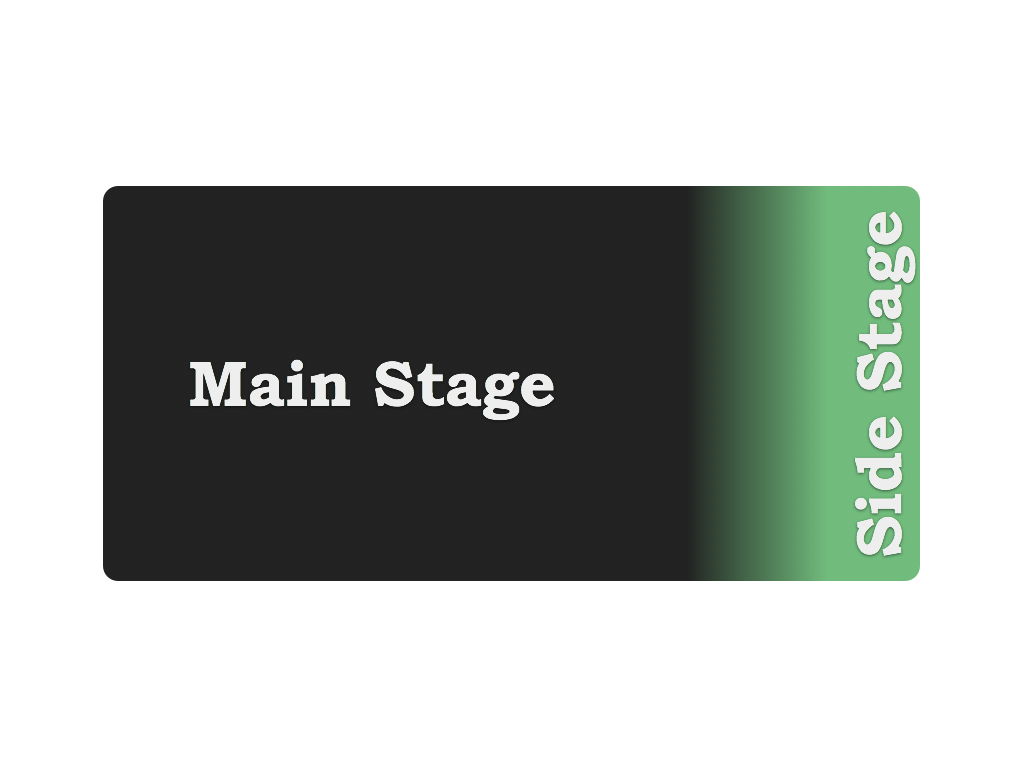
\includegraphics{figures/main-side-final.png}
	\caption{The final conceptual model that I argue for. Main and side stage are well blended and can influence each other. Main stage and side stage share an audience.}
	\label{fig:main-side-stage}
\end{marginfigure}


Although Goffman's description of appropriate performances for a specific audience is valuable, we want to avoid that front-back distinction enacted in the restaurant. Instead of having separate audiences, we want to create a space where, although the modes of performance are different, the performances are available to everyone. While in a channel metaphor, audiences are split between multiple back channels which are largely unavailable to someone performing on the front channel, stages create the opportunity for situations where the audiences for each stage can be shared. This unified audience helps us move away from the front/back distinction to a main/side distinction. In this model, performances on the main or side stage both share one large audience. By unifying the audiences, we can help avoid the problem with backchannels where they tend to assume a covert character. If side stage participation is accessible to everyone, it changes the character of the communication. Side stage performances lose some of their covert nature because they can be seen by a larger audience that includes main stage performers. Simultaneously, main stage performers can be made actively aware of side stage performances in a way that is inclusive, to help them better react to their now more present audience.

To reiterate, this change in metaphor has two components: a shift from channels to stages, and a shift from front/back to main/side. This is an aspirational shift; most of the design work in this space to date has represented the backchannel approach. But if these systems are to be an effective addition to face-to-face-type experiences, I will show how adopting this new metaphor can create effective communication experiences that encompass multiple simultaneous opportunities for engagement that create an effective, unified experience. This final configuration is shown in Figure \ref{fig:main-side-stage}. 

% Each is a performance, but the backstage is presumably more authentic. So unlike the concept of channels, which are composed of discreet information streams, stages are negotiated sites of performance around a singular situation.

% Instead of the metaphor of channel, he would refer to these alternate communication streams as stages.  When one moves from formal interactions to less formal interactions, one moves from front to back stage. When on the front stage, performance is prescribed and specific roles can be rigid.  And when on the back stage, one is more free to authentically represent themselves and their thoughts about the front stage.  He uses the example of a waiter behaving one way with a customer and then walking into the kitchen and telling the cook about the customer's difficult behavior.  Each is a performance, but the backstage is presumably more authentic. So unlike the concept of channels, which are composed of discreet information streams, stages are negotiated sites of performance around a singular situation. 






% This shift from 
% 
% 
%  But in a seminar environment, attentiveness and participation are more scrutinized because of the size and nature of the group. This suggests that integrating new communication technology into groups of smaller size might be more challenging because \emph{going away} is more difficult to politely incorporate into the front stage performance.  
% 
% 
% Communication systems used in a context where they are not the primary communication channel have historically been referred to as ``backchannel'' communication systems. Chat-oriented systems were the most popular, and have been deployed in a variety of contexts, though research has often focused on  conferences \citep{mccarthy_digital_2004, Rekimoto:1998jy} and classrooms \citep{Cogdill:2001fp,Yardi:2006uk} as fertile spaces for these sorts of interventions. More recently, tools like \emph{Twitter} have been described as a ``backchannel'' for live events. In some cases, a live-updating feed of recent tweets containing certain event-specific keywords have been projected in the space.
% 
% Although my work seems at first glance to fall into this same category of backchannel designs, I argue that a shift in the categories we use to think about these systems is important for building effective spaces. 
% 
% 
% 
% 
% In the literature about mediated communication systems used in a context where they are not the primary channel

 % Need to introduce stages as a concept here! Do the whole backchannel -> side stage transition argument here? It has to happen somewhere and it has to happen EARLY. It doesn't happen anywhere in background yet. 


\section{Design Spaces, Themes, and Theory}

One of the challenges of building technical systems as research is understanding the scope of conclusions. If you took a particular design element into a different system, would it operate in the same way? What are the relationships between the sorts of people using the system and the socio-technical structures that emerged? These are difficult questions to answer within the scope of a single project. The researcher may have solid intuition, but the tendency of the researcher is probably to see overly-general results more often than overly-specific results. One of the ways I address this is by describing a series of projects in this design space and examining design elements and themes in a variety of contexts.

This would be less effective as an approach if each of the design spaces was quite similar. The contexts I am designing for can be organized around a series of major differentiating axes:

\begin{description}
\item[Main Stage]{The medium for the main stage, e.g. the site of the primary shared experience of the audience.}
\item[Shared Display]{The presence or absence of a shared display.}
\item[Side Stage Attention]{The frequency of audience attention on the side stage. This is quite qualitative and varies across users, but each system embeds contains certain assumptions about the relative importance of the side stage to the main stage.}
\item[Audience Size]{The target audience size for the system.}
\end{description}

Table \ref{tab:project-axes} lists the research contexts covered in this dissertation, and describes each project's location on the major context axes. The variety across these axes helps show the breadth and scope of my work. 
\begin{table*}[tb]
	% \centering

\begin{tabular}{r|llll}
& Main Stage & Shared Display & Side Stage Attention & Audience Size \\
\hline
\textbf{backchan.nl} & face-to-face & yes & infrequent & 20-500 \\
Information Spaces & virtual world & yes & infrequent & 10-20 \\
ROAR & broadcast video & no & frequent & > 1,000 \\
\textbf{Tin Can} & face-to-face & no & occasional & 10-20 \\
\end{tabular}
\label{tab:project-axes}
\caption[][15pt]{Comparing the projects covered in this dissertation on the major axes that distinguish them. Projects in bold are major projects discussed in the most depth. Small project variants (e.g. backchan.nl for remote Q\&A, Tin Can Meetings, etc.) are not included.}
\end{table*}

% could I identify a set of common design elements that can be traced across all projects?
% voting
% chat
% shared display?

Although each project operates in a different context, there are a number of research themes that each project addresses. Although these themes were not identified at the start of this research stream, they nonetheless are present in all my work to various degrees. It can be challenging to identify the broader impact of design-based research (a topic I will address in more depth in the next chapter), but it is through looking at these themes in different contexts that I hope to contribute to broader discussions. These are themes that are relevant particularly to designing complementary interfaces like those in my own work, but also to many kinds of collaborative, synchronous systems, even those which aren't trying to create complementary experiences.

\begin{description}
	\item[Grounding]{My work uses shared displays in a variety of different capacities. I contend that these kinds of public displays can play a powerful role in helping to ground, in the \citet{Clark:1989uc} sense, a conversation. In particular, shared displays can provide ways to non-verbally acknowledge discourse presentations. By their very shared nature, the contents of shared displays might accelerate the creation of common ground. The different ways that these shared displays operate in my work helps provide insight into both particular design techniques to support grounding as well as the broader discussion around how common ground operates in mediated communication contexts.}
	\item[Non-verbal actions]{As a result of the drive to create a sense of ``being there'', mediated interaction systems failed to consider the ways that we communicate non-verbally, assuming that higher fidelity video and audio would be sufficient to capture that communication. I contend that our non-verbal actions in the physical world are a critical component of body language, and when creating mediated channels we should strive to create new vocabularies of action that enable people to communicate non-verbally. In much the same way that in a shared physical space we can observe people interact with objects around us, so too should people's actions in mediated systems be visible and part of supporting a sense of presence and awareness. How these action vocabularies are constructed and communicated to people is critical to the success of these sorts of systems.}
	\item[Attention]{Creating new opportunities for simultaneous commentary and communication about some shared experiences creates situations where people have to make choices about which if the stages to attend to and which stage to use for their performances. From a design perspective, there are a number of important attention related decisions to make: How is our attention made visible to others, and how does it affect their impressions of us? How do we design displays for occasional attention of users who are shifting their attention between different stages? Understanding how people think about and enact attention in situations with multiple available communication channels is critical to designing appropriate options and understanding the practices that evolve around them.}
\end{description}

This work contributes on two levels. First, by creating and deploying interfaces with particular properties, I provide concrete guidance and insight about particular specific design strategies and interfaces. This is valuable for designers and researchers thinking about how they design this variety of communication systems. I also contribute to the broader discourse about the three research themes laid out above. In each case there are both broader theoretical contributions to be made as well as specific findings that contribute to scholarly discussions about these issues.

\section{Thesis Organization}

This thesis starts with a broad background discussion about some of the methodological assumptions implicit in doing design work as research, a tour through some of the high level related work that all of my work relies on, and a more in-depth treatment of the major research themes I introduced here.

Based on this background, I will then discuss four major project areas in each of the following four chapters: Virtual Worlds (which contains two specific sub-projects for meetings and presentations in virtual worlds), \emph{backchan.nl} (a tool for managing audience feedback during live events), \emph{Tin Can} (a tablet-based platform for enhancing small group discussions), and \emph{ROAR} (a platform for very large scale audience interaction during live events). Through each of these chapters I will relate my findings back to the research themes that are laid out in Chapter \ref{ch:background}. 
\chapter{Background}

%intro to the background section here





% : virtual worlds, face-to-face panel discussions, small group seminar discussions, business meetings, remote information sessions, and live-event spectating

% Part of what's attractive about mediated communication systems is that there is a tremendous variety of ways to design and use them once we set aside a desire to recreate face-to-face interaction. Although in this section I've contrasted mediated communication with face-to-face communication in a way that might imply that mediated communication systems are somehow monolithic and self-similar, the survey of related systems in the section to follow will illustrate the tremendous range of potential systems in this space and demonstrate how thoughtful designs can have widely varying impacts on the experience of communication or collaboration. 

% My work takes this general design strategy of adding new communication channels in a few different directions. In this proposal, I will describe my past work looking at meetings in virtual worlds, audience-speaker interaction in presentations, and classroom discussions. I will also lay out my design for a system to support face-to-face meetings with remote participants. These research contexts vary both in the numbers of simultaneous participants, as well as their geographic configuration. Over the course of my work, I have shifted my attention from configurations where all users are remote (\emph{Information Spaces}) to heterogeneous situations where some or all of the participants are co-located (\emph{backchan.nl}, \emph{Tin Can Classroom}, \emph{Tin Can Conference}). 

% TODO Add a paragraph here that preludes some of the design as research ideas (which will be covered in more depth in their own section) as a way of saying that having these themes is part of what makes this research-worthy. 

\section{Design as Research}
% there are a few points here. 
% 1. a broad introduction to design as a valid research strategy
% 2. projects I did, and the coverage of the space
% 3. themes and theory

Proposing a design space and arguing for its value as an approach to common problems is not, traditionally, the realm of academic research. It is a frequently taken-for-granted assumption at the Media Lab that designing novel technical systems is a natural and defensible way to do research, but outside of that context this may seem like an unusual way to conduct research. Given that this assumption is fundamental to this work, it seems productive to address this question from the start. Design as research is clearly being conducted in a variety of contexts using a variety of methods, yet there is very little discussion or agreement about the fundamental aspects of how that work is conducted and what we can learn from it, let alone a positive argument for why it might be the \emph{best} approach for certain kinds of research questions. It is frequently tolerated but not actively advocated for. 



Because my research practice uses design and development as its primary research method, it seems productive to describe explicitly why this is a valuable research approach. I will describe the sorts of contributions one can make working this way and contrast this approach with other approaches dominant in the fields of human computer interaction, computer mediated communication, and computer supported cooperative work.

% TODO This is a stupid title, especially relative to the section title. FIX IT.
\subsection{Engineering as Research}

% can I get away with these claims? if I wanted to be serious about it I would do a some lit review statistics. but I don't really want to get bogged down in that. Lets see if I can get away without it.
It is a gross simplification, but let us separate work in these fields into three general categories: technology-enabled sociology and psychology, studies of systems in-the-wild, and design of new systems. In the first category, researchers seek to answer the kinds of questions typically of interest of sociologists and psychologists, but deploy technology to allow them to be answer questions have not been able to answer in sufficient detail in the past. This work focuses primarily (but not exclusively) on drawing conclusions about the behavior and experiences of either individuals or collections of people. Studies of systems in-the-wild are, in contrast, more focused on understanding the relationship between the technology and its use, often described as the socio-technical system. Finally, there are researchers who design and build novel systems and then study them. I describe this final category of researchers (in which I consider myself a member) researchers-as-designers. 

These last two categories are deceptively similar. After building a novel system, does one simply run a study on that system like a researcher who didn't build the system themselves? This suggests a critical thought experiment: if the researcher-as-designer could simply imagine a system into existence that looked exactly like the system they wished to study, would that compromise the research in any fundamental way? Put another way, does the actual design and implementation process actually add value to the research or is it just an overhead?

There are two ways to address this issue. First, the thought experiment is subtly mis-framed. Technical artifacts can never really be imagined into existence because their creation is a constant negotiation between the properties of the tools used to create it, the environment in which the design happens, and the reactions the designer has to their own work. In practice, the artifact that comes out of a design process is the result of a lengthy iterative process, even in design processes that don't conceive of themselves as iterative. Simply creating part of an artifact and integrating into another part causes a re-evaluation of those parts in a way that causes designs to drift from their original models. The time spent in the design and implementation processes can be seen as critical for producing a viable design. If we desire to study systems that don't already exist, there is simply no way around spending time on the design itself because our ideas about what the design could or should be before entering those process can't really become real, and if they could they would be unlikely to meet any of the original design goals. From this perspective, we view the development process as a fundamentally necessary cost of creating any novel system. 

% took this from some older writing I did - don't need to dig into that particular account because readers other than Wanda won't be familiar with it.
% The second approach is to turn to Schutlze's confessional account of her dissertation field work in which she struggled with the practical realities of trying to be a participant in the work lives of her informants without injecting her own in-progress conceptualizations of their work experience and without her researcher identity becoming compromised by her affiliation with a specific work group in the organization. Yet, we (I think rightly) value her attempts to not simply sit outside the process she's studying, but to take part in it. This is fundamental to participant-observation as a methodology. 

The second approach is to consider the distinctive values of the design process as a research process. In some fields, we expect that the researcher will become deeply embedded in the process on which their work focuses. In these fields, putting yourself at a distance and insisting that you can simply observe without being part of that process is often viewed as naive. Yet when we shift our focus to creating novel technical artifacts, we prefer to isolate either the users (as in lab studies) or the treat the artifact itself as stable (as in studies of the use of existing artifacts \emph{in situ}). It seems only natural to say that claims about the design of socio-technical systems can be easily augmented by a long-term, rich participation in that exact process. Playing the role of the active participant in the process grants us credibility and real analytical leverage. Not to say that you can't make arguments about design choices of a technology without having been part of the team that made them--you certainly can—-but being a participant in that process provides important insights that we are unlikely to find if we treat the technology as the black box output of an historical design process conducted by others. 


% this paragraph needs to be about WHAT ARE THE INSIGHTS FROM THE DESIGN PROCESS?

It is difficult to precisely identify the sorts of contributions that would not be possible without engaging in the design process because there are few examples of a team doing novel design work and handing off the result to a separate researcher and comparing their results. We do have a large body of research on systems conducted by non-designer researchers, but there's nothing to systematically compare it to. I hope that my work highlights how the researcher-as-designer can operate effectively in both roles and serve as a starting point for a broader discussion about why designing and studying systems is as valuable a research strategy as studying existing systems. \sidenote{Designing and building systems can take a substantial amount of time, especially if you hope to deploy those systems \emph{in situ} instead of in lab contexts. If papers are the main output metric for a researcher, this approach is not necessarily an efficient way to generate papers, since few conferences will accept papers on the design or development of a novel system alone. This might help explain the waning popularity of this sort of research.}

If we accept that conducting design and development are valuable research processes, we must consider the challenges to this kind of work. If we hope to avoid the limits of studying design work in decontextualized lab situations, then we need to find situations were our system might credibly be used ``for real.'' The best situations are ones in which people interacting with and through the system can do so in the normal contexts in which they might interact with such a system: using their own devices, in places that are familiar to them, and with people who they might normally use such a system with. These contexts can be quite difficult to secure. Some systems require a certain scale to reveal meaningful results; had a researcher designed Twitter, they would have been very hard-pressed to find a context in which they could study it in a legitimate way. These constraints are also acute when designing for business contexts. Deploying research software in business contexts poses risks for the business in terms of data security as well as ethical concerns about businesses compelling their employees to use the system. Although this limits the kind of design work the researcher-as-designer might credibly study, these constraints are notably different than the constraints on researchers who study existing in-the-wild systems. In many ways, these biases are nicely complementary:

\begin{table}[tb]
\begin{tabular}{r|l}
\textbf{Researcher-as-Designer} & \textbf{Researcher} \\
using novel technology & using existing technology \\
not widely deployed or available & popular/widely used \\
smaller, bounded user groups & larger, fluid user groups \\
extrinsically motivated users & intrinsically motivated users\\
rougher edges & well polished\\
consumer-oriented & consumer or professional\\
bounded use durations & potentially unbounded use durations\\
internal process traces & publicly observable process traces\\
\end{tabular}
\label{table:research-focus-comparison}
\caption{Comparison between the kinds of technical contexts that the researcher-as-designer typically studies compared to the researcher.}
\end{table}

On most of these axes, it is not that researchers are incapable or uninterested in studying the kinds of systems that the researcher-as-designer studies, but that (for a variety of systemic and historical reasons) they have gravitated towards these themes. Whatever the reason, these differences add to the value of the researcher-as-designer approach. Even if taking the role of researcher-as-designer takes a substantial time investment to create the systems being studied, if it reveals insights about new kinds of systems that traditional researchers might not pay attention to, then it can be a valuable approach. This is most true with respect to the properties of the technology in the system. The researcher-as-designer can also be conceived of as mapping terrain that the designer-as-professional and other researchers will later cover when the technology becomes more widely accessible or viable. Furthermore, the kinds of deep data collection possible with custom-engineered systems open up a variety of analytical options that are often not possible when trying to collect data from publicly available and usually corporate-controlled contexts like Facebook or Twitter.

\section{Methodology}
% ??? Could talk about studies in authentic contexts and do the whole critique of lab-based studies here. Probably not super relevant, and a bit risky since a lot of the stuff I'll end up talking about doesn't have particular studies attached to it. 

% other potential topic: broad ideas about how people and technology interact and what the focus of study is?


\section{Related Work}
Designing new systems for collaboration and communication, as opposed to studying existing systems, has long been a major stream of HCI and CSCW research. This section will summarize the most salient past work in this area, although little of this work is recent and responsive to the significant shifts in the way people use technology to communicate, collaborate, and play. 

For a variety of reasons, there has been somewhat of a shift in interest away from the kind of hybrid face-to-face/mediated experiences I create towards building and studying systems for asynchronous experiences between much larger numbers of people. The advent of research on mass collaboration systems like \emph{Wikipedia} (e.g. \citep{Kittur:2007up}) and ``crowd sourcing'' (e.g. \citep{Bernstein:2010wk}) is part of a larger shift away from what was once the center of gravity of systems research. This shift is a natural response to changes in both technology and the common experience of modern collaborative technology users in a web-oriented world where asynchronous interaction became the norm. But the experiences this sort of research studies focus on are predominantly single-channel and asynchronous. This is in stark contrast to my work, which is concerned with the properties of multi-channel synchronous experiences. 

In this work, I focus on interactions within groups both small and large, co-located and remote, but always co-temporal. Although interesting new sorts of work and communication structures are evolving in the asynchronous domain, we should think not just about how to marshal large numbers of people, but about how small groups of people who know each other work, recognizing that much of that work happens face-to-face or co-temporally while geographically distant. It is not effective to treat these interactions as a simple increase in tempo on asynchronous interactions. In synchronous systems, it is much more important to understand how we are perceived (and can control those perceptions) by others. In asynchronous systems, these issues are minimized; we experience others through their actions on shared objects like documents. 

% In my work, I seek to create richer representations of people and better-support person-person interaction instead of person-document-person interaction. 

My survey of related work is organized into three major design strategies: translucence and awareness, adding new communication channels, and design techniques to help people reflect on their own participation and the participation of others. These design strategies have influenced my own design process and have important findings related to my three main research themes: grounding, actions, and attention. As I discuss each design strategy, I will point out their connections to the main research themes. Table \ref{tab:related-work} summarizes the major work covered in this section, and its relationship with the three themes. 


% TODO think about whether to add in a chunk about theoretical perspectives here. Ultimately in the final dissertation there will need to (probably) be a chapter or serious chunk of one laying our theoretical perspecives on grounding, attention, and non-verbal actions. But I don't really want to have to do that now.


% do the table here
% \bullet \medbullet \cdot \filledcircle \filledbigcircle


% c c c c c c c c c c c c c c c c c c c c c

\begin{table*}[tb]
	% \centering

\begin{tabular}{lrcccl}

& & \begin{sideways}Grounding\end{sideways} & \begin{sideways}Actions\end{sideways} & \begin{sideways}Attention\end{sideways} \\
\midrule


\multicolumn{2}{l}{Social Translucence} & & & & \\
\midrule

& \emph{Loops, Babble, Lecture} &$\bullet$& $\CIRCLE$ & $\cdot$ & \citep{Erickson:2000kb} \\
& \emph{Group SketchPad} &$\bullet$& $\CIRCLE$ &$\bullet$& \citep{Gutwin:2002tf} \\
& \emph{CafeCK} &$\bullet$& $\CIRCLE$ &$\bullet$& \citep{Ackerman:1995tj} \\
& Airplane Cockpits & $\CIRCLE$ & $\CIRCLE$ & $\CIRCLE$ & \citep{Hutchins:1995ud} \\
& \emph{ClearBoard} & $\CIRCLE$ &$\bullet$& $\cdot$ & \citep{Ishii:1992bq} \\
\midrule


\multicolumn{2}{l}{Channels} & & & & \\ \midrule & Class Backchannels &
$\cdot$ & $\cdot$ &$\bullet$& \citep{Yardi:2006uk} \\ & Conference
Backchannels & $\cdot$ & $\cdot$ &$\bullet$& \citep{mccarthy_digital_2004} \\
& Semi-Public Displays &$\bullet$&$\bullet$&$\bullet$& \citep{Huang:2003ef} \\
& \emph{Rendezvous} &$\bullet$&$\bullet$& $\cdot$ &
\citep{kellogg_leveraging_2006} \\ & Audio Backchannels & $\cdot$
&$\bullet$&$\bullet$& \citep{Yankelovich:2005bx} \\ & Fragmented Social Mirror
& $\CIRCLE$ & $\bullet$ & $\bullet$ & \citep{Bergstrom:wl} \\ &
\emph{VideoWindow} &$\bullet$& $\cdot$ &$\bullet$& \citep{Fish:1990fn} \\ &
\emph{Thunderwire} & $\cdot$ &$\bullet$& $\CIRCLE$ & \citep{Hindus:1996cn} \\
& \emph{iCom} &$\bullet$&$\bullet$&$\bullet$& \citep{Agamanolis:2003wc} \\ &
\emph{Portholes} &$\bullet$& $\cdot$ &$\bullet$& \citep{Dourish:1992fu} \\ &
\emph{Cruiser} & $\cdot$ & $\CIRCLE$ &$\bullet$& \citep{Fish:1992vz} \\ & GDSS
& $\CIRCLE$ &$\bullet$& $\cdot$ & \citep{nunamaker_electronic_1991} \\ &
\emph{Cognoter} & $\CIRCLE$ & $\CIRCLE$ & $\CIRCLE$ & \citep{Tatar:1991jq} \\
\midrule \multicolumn{2}{l}{Reflection} & & & & \\ \midrule & \emph{Second
Messenger} &$\bullet$& $\cdot$ & $\cdot$ & \citep{DiMicco:2007ie} \\ &
\emph{Meeting Mediator} &$\bullet$& $\cdot$ & $\cdot$ & \citep{Kim:2008ip} \\
& \emph{Conversation Clusters} &$\bullet$& $\cdot$ &$\bullet$&
\citep{Bergstrom:2009fe} \\ & \emph{Conversation Votes}
&$\bullet$&$\bullet$&$\bullet$& \citep{Bergstrom:2009ej} \\ &
\emph{Conversation Clock} &$\bullet$& $\cdot$ &$\bullet$&
\citep{Bergstrom:2007je} \\ \bottomrule \end{tabular} \vspace{3em} \caption{A
summary of the major related work to be discussed in this section and its
relationship with the main research themes. } \label{tab:related-work}
\end{table*}

\subsection{Translucence \& Awareness}

This work owes a clear debt to the work of \citet{Erickson:2000kb} on social translucence. Their work intersects with my action and grounding themes. \emph{Social translucence} is a design strategy that aims to create ``digital systems such that people's presence and activity, made appropriately perceptible, will create accountability and more easily coordinated action''  \citep{Kellogg:2002ts}. They call their example systems designed for this purpose ``social proxies'' that use ``abstract visual representations ... to portray information, in addition to contextual information provided by the other common traces of user activity in mediated communication environments (e.g. persistent conversation).'' In each of their projects (Babble, Loops, Lecture, Auction, etc.; \citep{Erickson:2003td} is a nice overview of these projects), they seek to promote a sense of ``collective awareness'' where each person using the system has a sense of the actions of others in the system and appreciates that this awareness is mutual. 

We share an interest, in my terms, in how we can construct meaningful actions in mediated social spaces and how we can understand how public displays can help ground collaborative and discursive processes. As Erickson and Kellogg point out, this has been a topic of interest both direct and indirect for quite some time in the systems literature. Their work nicely complements work by \citet{Gutwin:2002tf}, who present a framework for thinking about the ways the workspace awareness through actions can be constructed and presented.  \citet{Ackerman:1995tj} shares this interest, too, but focuses on representing overall system activity as an inducement for broader participation. This is an important finding, and one I echo in my work, particularly when it comes to a public, optional system like \emph{backchan.nl}. Distributed cognition, as described by \citet{Hollan:2000ud} represents another productive way to think about these processes; by fostering a sense of mutual awareness we can supporting the kinds of process that \citet{Hutchins:1995ud} describes in flexible communication systems. I see my work as a continuation of these past approaches to representing activity. Although there are many similarities in terms of findings and design strategies, I will focus here on the points of difference as a way to clarify the contributions of my work.

\begin{marginfigure}
	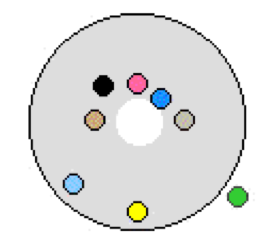
\includegraphics{figures/babble.png}
	\caption{Screenshot of Babble, showing high activity users (in the center) and lower activity users (around the edges), from \citep{Erickson:2003td}.}
	\label{fig:proxy-babble}
\end{marginfigure}

Although Erickson and Kellogg are particularly concerned with what is made visible and what is kept private (the difference between, in their terms, \emph{transparency} and \emph{translucence}), this is a point of divergence between our work. Although I agree with their analysis of the value of considering what actions should be made visible and what should be concealed, it is not a main focus of my analysis. In my work, reading is essentially always invisible and any other action is visible. This is partially a response to their suggestion that it is ``important that participants were aware of the others' awareness of [the properties of the system]'' \citep{Erickson:2003td}. This fits nicely with \citet{Brennan:1991wk}'s presentation of grounding. Simply being told something by someone is not enough for the conversation to move on - you must accept that presentation of information, and that acceptance needs to be accepted by the original presenter. In this way, grounding plays a role not just in communication itself, but in how we communicate information about who we are and what we're doing through actions in the system. 

This finding also suggests that if you don't know which actions are public and which are private, it diminishes the value of translucence as a design strategy. In their work, they tend to rely on physical metaphors to communicate the visibility properties of a system. This is a sensible strategy, but I feel this limits the kinds of experiences we can craft. In my work I tend towards not including invisible actions and instead create completely transparent spaces with carefully selected actions that are worth making visible. This is possible partly because the group sizes in my work are smaller than in the main examples they propose, and it's feasible to show all actions without it being overwhelming. 

\begin{marginfigure}
	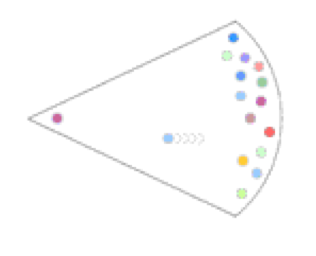
\includegraphics{figures/lecture.png}
	\caption{Screenshot of the lecture proxy, showing the speaker on the left, students on the right, and an interrupting student moving towards the left, from \citep{Erickson:2003td}.}
	\label{fig:proxy-lecture}
\end{marginfigure}

They share a number of specific design findings that complement some of my experiences designing similar systems. They describe three approaches to visualizing activity: realist, mimetic, and abstract. \citep{Erickson:2003td}. I share their interest in abstracted representations, although for different reasons. They argue that realist and mimetic approaches face ``substantial pragmatic barriers (e.g. expense, infrastructure, support)''. In the years since this work was originally done (and well before; one might reasonably argue that \emph{ClearBoard} \citep{Ishii:1992bq} represents an elegant realist approach), many of those pragmatic barriers have fallen. We've seen large-scale virtual worlds (like \emph{Second Life}) that used mimetic approaches and wide adoption of video conferencing which uses realistic representations. Instead, we argue that abstract representations are simply more flexible and better, even given the option of realistic or mimetic approaches.


My work goes into greater depth than Kellogg and Erickson's does on the issue of ``public not personal'' displays. While we agree that it is critical that each person's display doesn't deviate in the kinds of information it represents, in my work these displays are not monolithic---they are not the only venue for interaction between people. Furthermore, displays in my work are most often themselves public, which reinforces the grounding effect. Indeed, that is the most significant deviation between our work. In all of the social proxy work, the proxy is the primary communication medium; in my work, my systems coexist with another primary communication channel, and rarely have any knowledge about the contents of that channel. Public displays also exacerbate issues of attention, which tend not to be major issues for work in the social proxy space (as shown in Table \ref{tab:related-work}). 

% put in a bunch of figures here of the social proxies they designed.



\begin{marginfigure}
	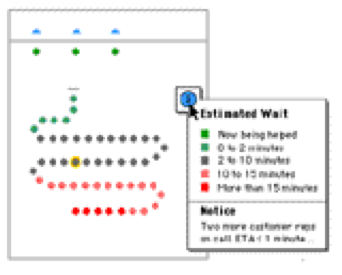
\includegraphics{figures/queue.png}
	\caption{Screenshot of the queue proxy, from \citep{Erickson:2003td}.}
	\label{fig:proxy-queue}
\end{marginfigure}

The other major distinction is in the use of metaphor and display techniques. Erickson and Kellogg box themselves in by limiting their representations to ``a relatively large geometric shape with an inside and an outside and sometimes other features that represent the online situation or context'' \citep{Erickson:2003td} with ``small colored dots'' to represent individual users (similar to \citep{Viegas:1999kv}, minus the direct agency). These design strategies are illustrated in figures \ref{fig:proxy-babble} and \ref{fig:proxy-lecture}. Furthermore, they argue that the best way to represent information is through the use of ``relative movement'' of the user-dots in a way that has ``metaphoric correspondence to the position and movement of people's bodies in face-to-face analogs of the online situation.'' \citep{Erickson:2003td} As I hope my work shows, these limits are not at all necessary to create spaces of meaningful action that facilitate grounded communication and collaboration. Specifically, the need for relying on face-to-face analogs is not a helpful constraint. Instead, my work seeks to create spaces that are easily understood and provide contexts for meaningful action without relying on existing face-to-face metaphors.



\subsection{Channels}

\begin{marginfigure}
	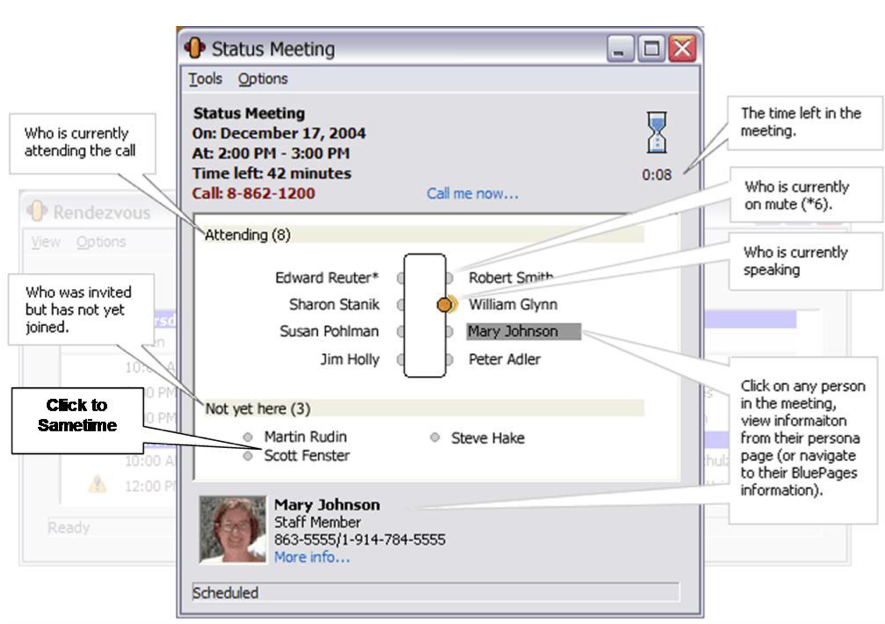
\includegraphics{figures/kellog_social_proxies.png}
	\caption{Screenshot of a meeting-room social proxy for promoting a sense of awareness of other meeting participants, from \citep{kellogg_leveraging_2006}.}
	\label{fig:social-proxies}
\end{marginfigure}

The primary focus of my work is on designing systems that add new communication channels and understanding how those channels operate in contrast to existing channels. In this section, I will present related work that addresses some of these questions.

\begin{marginfigure}
	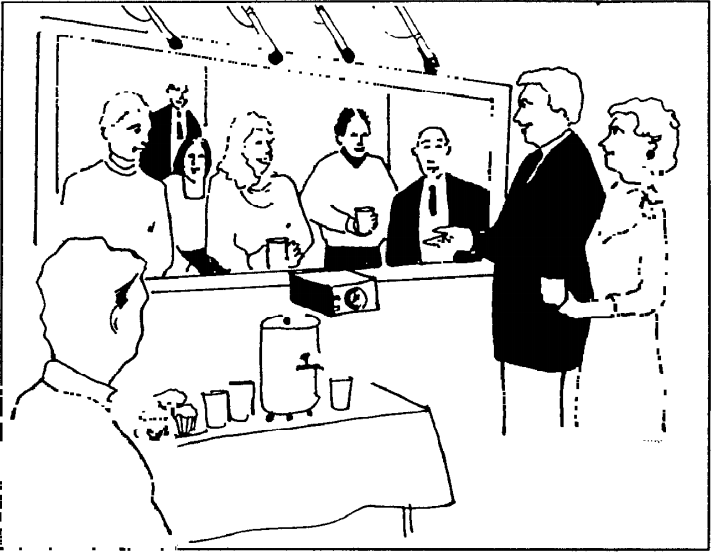
\includegraphics{figures/videowindow.png}
	\caption{Diagram of the VideoWindow scenario for connecting two work-place social spaces, from \citep{Fish:1990fn}}
	\label{fig:videowindow}
\end{marginfigure}

The work most directly related to these questions comes from research into so-called ``backchannels'' in presentation and classroom settings. \citet{Yardi:2006uk} describes how a chat-based backchannel operates over a semester in a classroom, \citet{mccarthy_digital_2004} describe a similar approach at a conference. Backchannels can also be considered a potential part of non-event-oriented contexts too, like long-term co-working among small groups. \citep{Huang:2003ef} Backchannels are not just focused on co-located groups, however, and \citet{kellogg_leveraging_2006} (among others, e.g.  \citep{Yankelovich:2005bx}) has addressed how text and audio backchannels can coexist in distributed contexts. Although past work has addressed in general terms the different ways people use backchannels, it has not sufficiently explained the complicated issues around channel selection, attention, distraction, and identity. Furthermore, in my work I try to move beyond just adding new text or audio channels by adding other kinds of non-verbal actions. In terms of my research themes, past work on backchannels has largely focused on characterizing use patterns, with some discussion of attention. More recent work, like \citep{Bergstrom:wl}, shares an interest in how we can construct actions and how shared displays can be used to help ground the interaction.

\begin{marginfigure}
	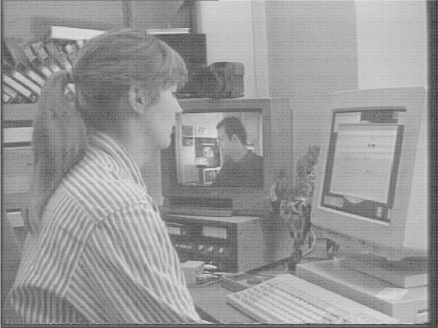
\includegraphics{figures/CRUISER.png}
	\caption{Photo of a CRUISER station installed in an office, from \citep{Fish:1992vz}.}
	\label{fig:cruiser}
\end{marginfigure}

\begin{marginfigure}
	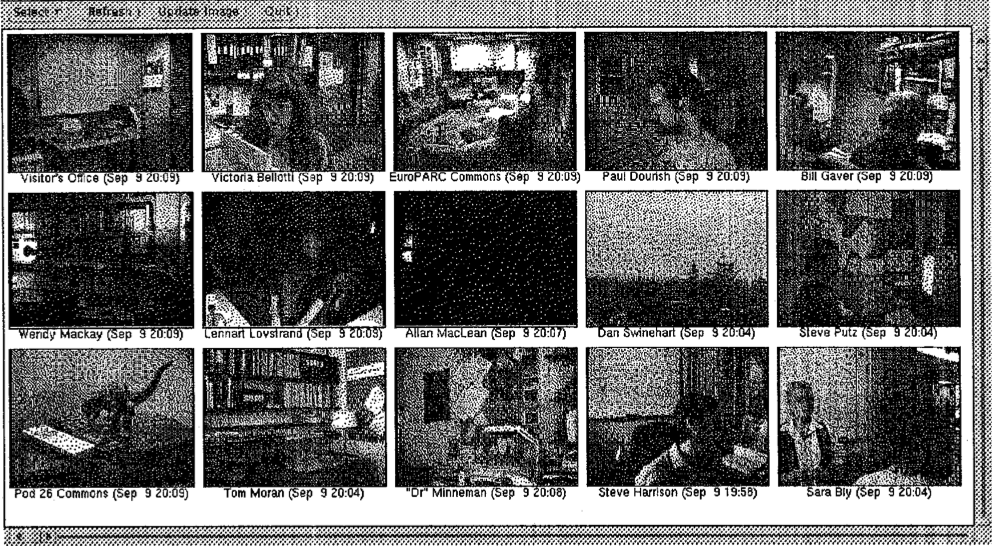
\includegraphics{figures/portholes.png}
	\caption{Screenshot of the Portholes interface, showing periodic stills from a wide range of environmental cameras in an office environment, from \citep{Dourish:1992fu}.}
	\label{fig:portholes}
\end{marginfigure}


Much of the work on creating shared media spaces, driven by experiments at PARC in the late 1980's and early 1990's is salient to my work. Although in some cases this work focused on creating new primary channels, researchers quickly became attuned to problems of privacy and attention because such systems always co-exist with face-to-face communication, in much the same way they do in systems I design. The earliest work at PARC \citep{Olson:1991vz} focused on creating flexible video connections between offices and conference rooms. Subsequent work focused less on a phone-call-like model where connections are created and ended and shifted towards creating spaces with different affordances. Sometimes these involved connecting multiple individuals together, as in CAVECAT \citep{Mantei:1991ww}; other times researchers focused on creating long term persistent video connections in common areas of distributed research groups in the VideoWindow \citep{Fish:1990fn} project. 


Over time, attention shifted more towards a taking advantage of the possibilities to do more than just create ``being there'' experiences. Some researchers experimented with audio-only spaces \citep{Hindus:1996cn}, finding that video was not required to create a sense of connection and space for users, but that the properties of audio did require audio-specific etiquette and coping strategies for the system to be useful. iCom represented a particularly rich design perspective on connecting spaces  \citep{Agamanolis:2003wc}, recognizing that awareness need not be limited to visual awareness, but can extend to information awareness which can be productively embedded in a media space. This embodies the ``beyond being there'' model best of all the work in this research stream: not just trying to create a transparent window between remote spaces, but making something better than a window could be. Furthermore, these projects also focus more on issues of attention, because they are not necessarily always the primary interaction venue for their users. 

% \begin{marginfigure}
% 	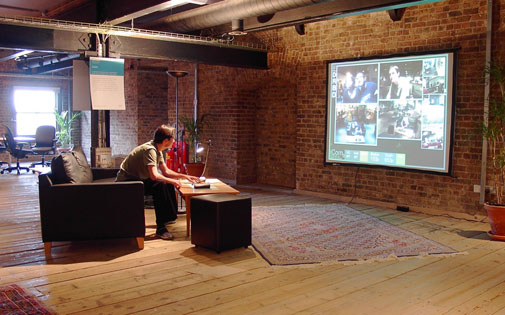
\includegraphics{figures/icom.jpg}
% 	\caption{Photo of one end of an iCom connection, showing multiple video streams and metadata along the bottom of the screen, from \citep{Agamanolis:2003wc}.}
% 	\label{fig:icom}
% \end{marginfigure}


\begin{marginfigure}
	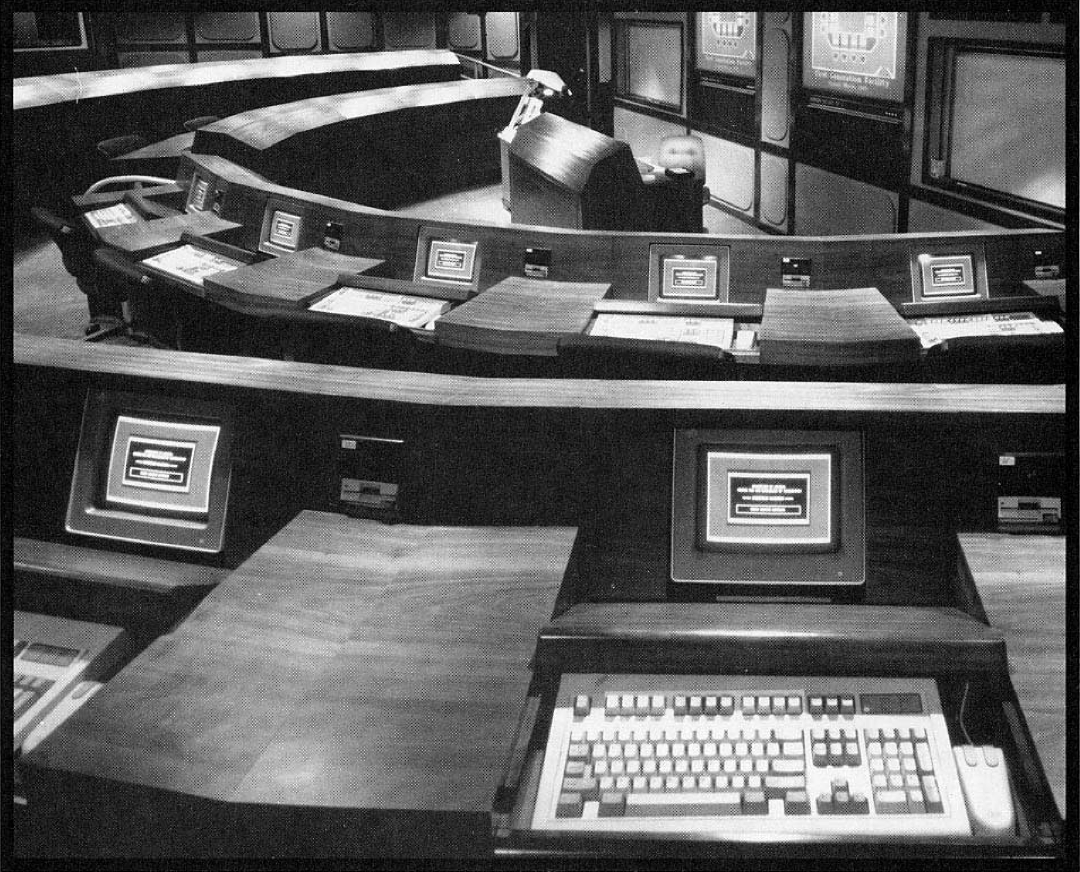
\includegraphics{figures/nunamaker_gdss.png}
	\caption{Photo of a GDSS space, from \citep{nunamaker_electronic_1991}.}
	\label{fig:gdss}
\end{marginfigure}


% also cite karrie's 
% (For subsequent, more artistically inclined approaches to this design space, see Karrie's blah blah, get a nice figure in here for that.)


Serendipity also evolved as an important part of sharing an office environment that was not present with most media space systems. Portholes \citep{Dourish:1992fu} addressed this explicitly by giving people a broader view of remote spaces instead of focusing just on main channel interactions. While my work is not concerned with serendipity, this kind of visual side channel carries important awareness information in much the same way that the side channels in my systems add important contextual information to an interaction. CRUISER \citep{Fish:1992vz} offered non-verbal ways to signal a desire to emulate some of the office hallway etiquette for signaling a desire to drop in and chat informally, without the explicitness of placing a call. The addition of moves like ``cruise'', ``glance'', and ``visit'' are similar in approach to the non-verbal actions at the core of my work like voting in \emph{backchan.nl}, promoting ideas in \emph{Tin Can Classroom}, or moving around the field in \emph{Information Spaces}. 

Early media space researchers proposed a distinction between ``formal'' systems from ``informal'' systems. \citep{Olson:1991vz} While most of the work discussed here (and much of my own work) tends towards the informal side of that continuum, there are some formal elements in my work. This formality manifests most strongly in Group Decision Support Systems research. These systems (exemplified by the work of Nunamaker \citep{nunamaker_electronic_1991}) provide prescriptive systems to support particular brainstorming, decision making, outlining, and voting schemes or policies. In the typical GDSS configuration, each participant has their own computer and interacts with shared structured data in some way, like submitting a new idea or voting on a proposal. In systems like this, the assumption is that having a structured display will ground otherwise informal processes by forcing participants to use the actions the system provides as a set of legitimate conversational moves. Although I tend towards informal systems in my work, the work in this space nonetheless has much to teach us about grounding and actions. 

The lack of consistent results in comparative work in this area \citep{Dennis:1988ww} illustrates the importance of focused design analysis to contextualize findings; it is not useful to view all brainstorming systems as equivalent and comparable in analysis, and I hope that my work will illustrate how the subtleties in interface and approach can have big impacts on outcomes that help explain some of the contradictory results in past GDSS work. Work in this space also raises serious questions related to attention that their work largely fails to address. In fact, in many situations they advocate for largely shutting down pre-existing primary communication channels to focus on the structured, mediated alternative.

Although somewhat rare in the literature, there are a handful of projects that directly address the kinds of hybrid spaces that I seek to create. \emph{Cognoter} \citep{Tatar:1991jq} addresses this design space most clearly. Like my work, \emph{Cognoter} created a hybrid space for very small groups (two to five people) that had both personal and public displays where users could create items and spatially arrange them like on a whiteboard. Textual items can be arranged on a users' display and that arrangement is mirrored on all other users' personal displays. The authors characterize \emph{Cognoter}'s model of creating shared text elements as representing a ``parcel-post'' as opposed to an ``interactive'' conversational model. Instead of embodying a present/accept process (as described by \citep{Clark:1989uc}), they describe their process as being more like literary communication (like email) where the writer tries to make sure ``that the addressees \emph{should have been able} to understand his meaning in the last utterance'' (emphasis mine). This is in contrast to face-to-face interaction, where we can interactively ascertain the extent to which we are being understood (and repair mistakes) before moving on. The authors describe \emph{Cognoter}'s failure to be used effectively by its users as (in part) a conflict between the interactive mode of face-to-face communication and the parcel-post model in \emph{Cognoter}. The \emph{Thoughtswap} project \citep{DickeyKurdziolek:2010wt} also shares my goal in creating hybrid spaces, but like \emph{Cognoter}, the mediated space is used serially with the face-to-face space, while I am interested in creating spaces for legitimate simultaneous performances in mediated and non-mediated spaces. This suggests a major hurdle for my work: can you create systems that use a parcel-post model yet still integrate fluidly with the interactive face-to-face model? \emph{Cognoter} and \emph{Thoughtswap} suggest this is hard, but I will show throughout my work how these barriers can be overcome and suggest ways to explain \emph{Cognoter}'s negative findings.

% go hunting for a desanctis and/or poole piece that's not focusing on AST specifically? also can hit berg if we want, but it feels like a bit of a distraction at the moment.

%, they also produced a nice taxonomy of the kinds of tools that would be useful for distributed collaborative groups: synchronous versus asynchronous communication and open processes versus focused processes, a distinction 


% there's a funny note in the portland paper about how they want to shift away from meeting augmentation to async and task coordination. Funny how times change.

% now summarize. 


% going to want to bring up media equation or whatever that book is called. Cliff Nass. 




% thundewire is just audio, basically a single-channel mumble. not so much about results as describing practices that evolved. 
% portholes is ambient awareness about remote places, not live interaction. cut it?
% videowindow is just like hole in space - audio/video fixed in space

% also mention virtual world stuff? MASSIVE might be worth a quick ref

% "shared media systems"

% - video projects like thunderwire + portholes
% - videowindow


% organize the work in this space 
% projects to talk about:
% - voiceloops
% - backchannel literature
% - social proxies
% - mention conferencing apps
% - Nunamaker
% - zephyr?


% \subsection{Theoretical Perspectives}
% thinking about leaving this out

% stuff from cscw paper:
% systems for reflection
% - second messenger
% - "social mirror" (Karahalios) also bergstrom
% - Meeting Mediator
% 
% systems adding new channels
% - (all the backchan literature: yardi, mccarthy, huang, kellog, yankelovich)
% - do a section on nunameker's work and why it's weird
% - 

% - we'll want to at the very least nod to thinks like voiceloops, and all the audio/video stuff like portholes and thunderwire and that kind of thing. farm my generals reading for that part.
%


% theoretical perspectives
% - practice lens?
% - ethnomethodology? 
% - re-farm wanda's reading list to see what else I can pull from there.

%
% We'll need to do a little organization here. Obviously, farm the references from the Tin Can Edu CSCW paper + backchan.nl paper. We'll need more, ofc, but it's a start. I suspect there will be some ways to separate out systems that allow communication versus those that simply reflect on a main channel. Maybe it's about whether the system itself is a single channel, multi channel, main channel or side channel? 

% write a methodological section here about why it's useful to study this with design work

\subsection{Reflection}

\begin{marginfigure}
	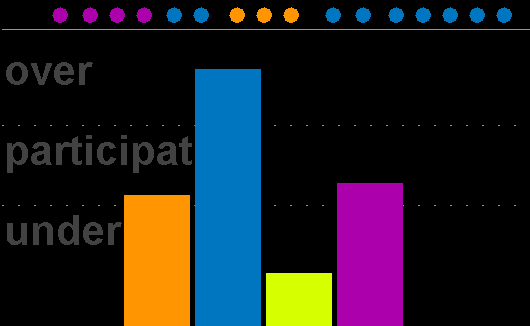
\includegraphics{figures/second-messenger.png}
	\caption{Screenshot of a Second Messenger participation bar-chart, from \citep{DiMicco:2007ie}.}
	\label{fig:second-messenger}
\end{marginfigure}

% \begin{marginfigure}
% 	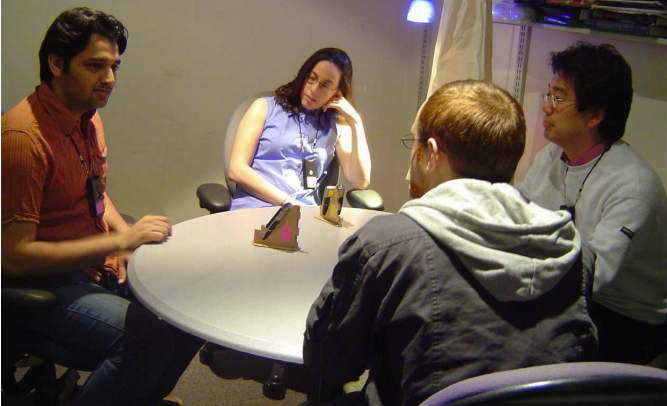
\includegraphics{figures/meeting_mediator.png}
% 	\caption{Meeting mediator.}
% 	\label{fig:meeting-mediator}
% \end{marginfigure}




Understanding how we present ourselves to others has been a topic of sociological inquiry for quite some time. Although many of the insights of scholars like \citet{goffman_presentation_1959} about how we communicate and interpret information about who we are and how we want to be treated are still relevant, the information that is available about people has changed substantially. In some of the examples in this section, designers have added some new bit of information about people to a face to face discussion; in others, we don't have any of the traditional information we would get from being face to face with someone and rely on new types of signals (like the non-verbal actions I propose) to create a sense of people around us. Part of what sets mediated communication apart is the ability to accumulate behavioral histories and represent and reflect those histories to ourselves and others. The work in this space is not as closely connected to my main research themes, but I include it here primarily because it has served as a source of design inspiration. 


\begin{marginfigure}
	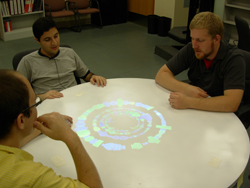
\includegraphics{figures/conversation_clock.png}
	\caption{Photo of Conversation Clock in use, showing relative participation histories from each conversation participant, from \citep{Bergstrom:2007je}.}
	\label{fig:conversation-clock}
\end{marginfigure}

My work is substantially inspired by the work of \citet{DiMicco:2007ie} on the \emph{Second Messenger} project. In this project, participants in a group discussion were presented with a constantly-updating bar-chart visualization representing the relative amount of time they had talked during the discussion. They found that while people who over-participated without a visualization tended to moderate their participation when the visualization was present, people with low participation did not participate more just because others were participating less. \emph{Meeting Mediator} \citep{Kim:2008ip} took a similar approach, but focused on situations where groups of two people could see each other and had to interact with another group of two people who they could only hear. Using a different visualization, Kim et al. found that groups were more interactive with the system than without, although there was not a correlation with group performance. 

\begin{marginfigure}
	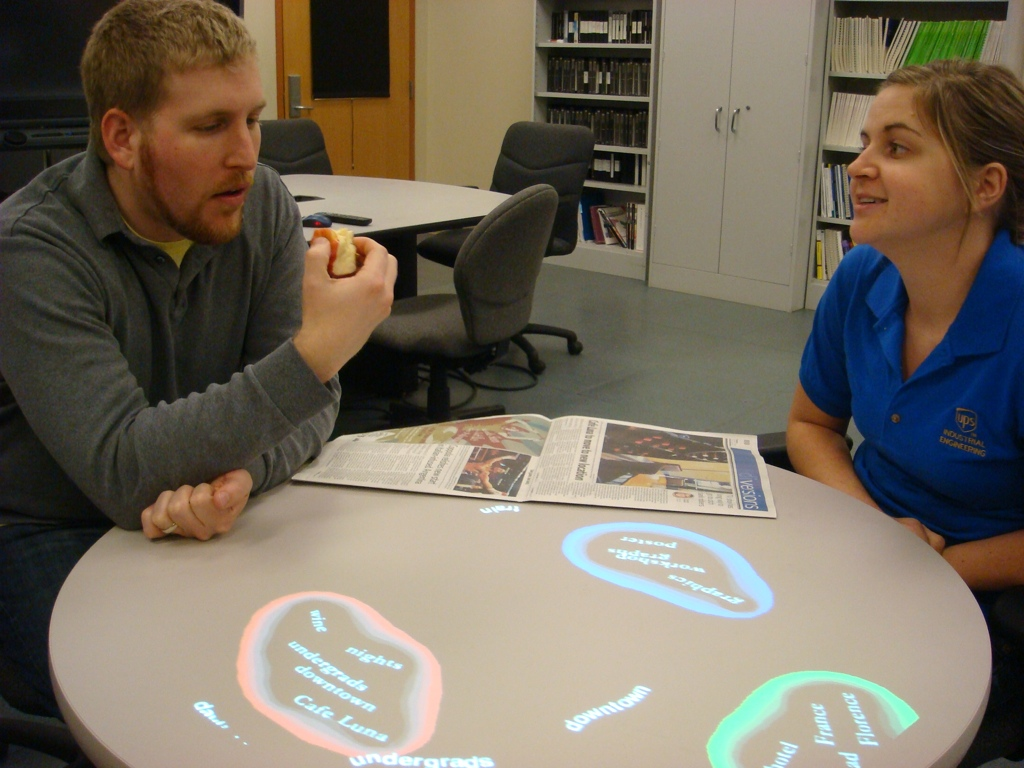
\includegraphics{figures/conversation_clusters.jpg}
	\caption{Photo of \emph{Conversation Clusters}, detecting audio themes and displaying them in visual clusters on the table-top display, from  \citep{Bergstrom:2009fe}.}
	\label{fig:conversation-clusters}
\end{marginfigure}


Bergstrom has done a series of projects that adopt a similar design strategy. \emph{Conversation Clusters} \citep{Bergstrom:2009fe} pulls topics from an audio conversation and presents them in clusters on a table-top display. \emph{Conversation Clock} \citep{Bergstrom:2007je}, like \emph{Second Messenger} and \emph{Meeting Mediator}, visualizes conversation participation, but uses a timeline metaphor instead of a aggregative metaphor. \emph{Conversation Votes} \citep{Bergstrom:2009ej} lets uses discreetly vote about the progress of a discussion, and displays anonymous votes on a table-based display. \citet{Karahalios:hu} describes this design space as ``social mirrors''. 

\begin{marginfigure}
	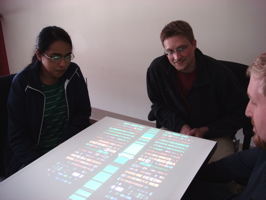
\includegraphics{figures/conversation_votes.jpg}
	\caption{Photo of \emph{Conversation Votes}, showing voting history among conversation participants on the table-top display, from \citep{Bergstrom:2009ej}.}
	\label{fig:conversation-votes}
\end{marginfigure}


% sneak in a \citep{visiphone} here?


% MATT TODO FIX THE MIDDLE OF THIS PARAGRAPH IT'S AWFUL
These are all examples of the accumulate and reflect design strategy, where the system tracks some aspect of behavior: spoken participation in the case of \emph{Second Messenger} and \emph{Meeting Mediator}, discussion topics and group attitudes in the case of Bergstrom's work. 

%The systems then present that information back to the individual or group with the intention that to reflect on and adjust their behavior. Furthermore, all of these projects have an element of grounding to them. By presenting this social information on a shared display (as in my work), it is made salient to the discussion in a way that private displays cannot.

% cite things like last.fm, goodreads, etc in this space?


% \subsection{Identity}

% maybe this whole section is dumb.
% how often do I really deal with this? It's clearly part of the second life work, but not at all part of backchannl, and only a little a part of the Tin Can series. Erm. Move on for now and double back. 

% Many other projects have focused on how peoples' identities are presented. In most of these pieces, there is no face-to-face element, which drives the researcher's interest in developing compelling alternative options that can richly communicate who someone is in a mediated space. Many informal and practical options are in common use; displaying an icon or image chosen by someone and a pseudonym to represent themselves is a widely used design strategy in social applications throughout the internet. These spaces for self expression are frequently augmented by systems that aggregate someone's behavior in that space. This is much like the reflection techniques, but are usually summarizing events beyond any single person's experience. The community site StackOverflow \citep{stack_overflow} provides a particularly rich example of this strategy.

% screenshot a wow forum, stackoverflow, 

% These techniques feel thin compared to the richness of face-to-face interaction, and researchers have developed a number of alternative approaches. Donath's work on data portraiture in a variety of 



% link to things like Ros' work in terms of augmenting face to face interaction with extra information? Or go back to steve mann's cyborg stuff?

% need a paragraph here that's more about the identity side of things. not sure what that will be. chat circles, perhaps? talking in circles? (whichever one had that intersting voting shapes thing)

% how to fit in social proxies and social translucense



% Other potential bits we could fill in here...
% We could spend some time with social translucense
% We could look at non-vebal actions as a space
%	start with Greenbergs stuff, but really look all over for groupware/collaborative tools that had some action to them. Will find some of that in the CVE literature, which might be easy to find
% I don't talk at all about theory stuff here. Could do the spiel about shared displays and grounding, but I'm not sure how critical that is going to be ultimately.
%
%
%  One other strategy is to think about the three research themes: grounding, non-verbal actions, and attention, and go on a hunt for good literature about each of those. 


\backmatter

\bibliography{dissertation}
\bibliographystyle{plainnat}

\end{document}



